\section{Retrieval selects evidence for an action}\label{sec:C16:objective}
Retrieval in an agent system is the selection of information that can change a consequential decision. The retrieved object may be a document passage, a temporal fact, a prior trajectory, a skill, or a tool description. These objects have different relevance criteria. A passage can support an answer without authorizing an action. A successful trajectory can suggest a procedure without proving that its preconditions hold now. Retrieval quality should therefore be defined relative to the decision and the role of the retrieved object.

Retrieval-augmented generation established a model in which generation conditions on external retrieved evidence~\cite{lewis2020rag}. That foundational formulation is not a description of every current agent-memory system. By the October 2026 cutoff, active graph traversal, state-conditioned trajectory retrieval, and runtime context construction make memory access a multi-step control process. The retriever and the reasoning policy can interact repeatedly rather than following a fixed retrieve-once-then-answer pipeline.

Let $S$ be the current task state, $D$ the available evidence store, and $Y$ the evaluation target. A retrieval policy $\rho$ selects $R=\rho(S,D)$ without observing $Y$. Let $\mathfrak R_A(S,D)$ contain the evidence subsets allowed by the current access policy $A$. For a fixed joint distribution of $(S,D,Y)$, a proposed objective is
\begin{equation}
 \begin{aligned}
 \min_{\rho,\pi}\quad &\mathbb E\!\left[
 \ell(a,Y)+\lambda C(\rho(S,D),S)\right],\\
 \text{subject to}\quad &\rho(S,D)\in\mathfrak R_A(S,D).
 \end{aligned}
\end{equation}
Here $a\sim\pi(\cdot\mid S,\rho(S,D))$ follows the actual deployed decoding and parsing law, and the expectation includes its randomness. The nonnegative resource cost $C$ includes search, reranking, context assembly, and generation; $\lambda\geq0$ converts that cost to the scale of the decision loss $\ell$. Missing-evidence consequences belong to the loss term. Relevance labels based on lexical overlap or passage entailment are proxies for this objective. They can be useful training targets without fully capturing whether the evidence changes the final action correctly.

The distinction matters for tool execution. An agent can retrieve the right account identifier but the wrong version of a permission policy. It can locate a valid example of an API call whose side effects differ from the present request. A retrieval metric that marks the identifier passage relevant can score the step as successful while the resulting tool call remains invalid. End-to-end evaluation should retain these roles and inspect the first decision at which the missing distinction matters.

Evidence also competes for a finite input budget. More retrieved items can increase recall while reducing the policy's ability to identify the authoritative ones. A retrieval system should report candidate recall, final evidence packing, and downstream use separately. A method that retrieves a decisive record but drops it during prompt construction has an assembly failure; a method that includes it but follows a stale conflict has an interpretation failure. Those distinctions guide different repairs.

For a specified decisive-evidence path, define nested events $E_1\supseteq E_2\supseteq E_3\supseteq E_4$: the required source is available and authorized, reaches the candidate set, survives packing with its qualification, and is appropriately used. When the conditioning events have positive probability,
\begin{equation}
 P(E_4)=P(E_1)\prod_{j=2}^{4}P(E_j\mid E_{j-1}).
\end{equation}
This is the probability chain rule, with no stage-independence assumption. It measures this evidence path, not all task success: another source or a different valid plan can bypass it. Conditional stage metrics expose a bottleneck that an aggregate recall score cannot locate. They should be estimated on the same workload cohort; multiplying rates from unrelated benchmarks is invalid. MRAgent, JAM, MATM, and MemCalib intervene at different factors, which is why their reported scores cannot be treated as interchangeable evidence of retrieval quality.



Figure~\ref{fig:C16:overview} isolates the mechanism and its stated information boundaries.
\begin{figure}[!htbp]
\centering
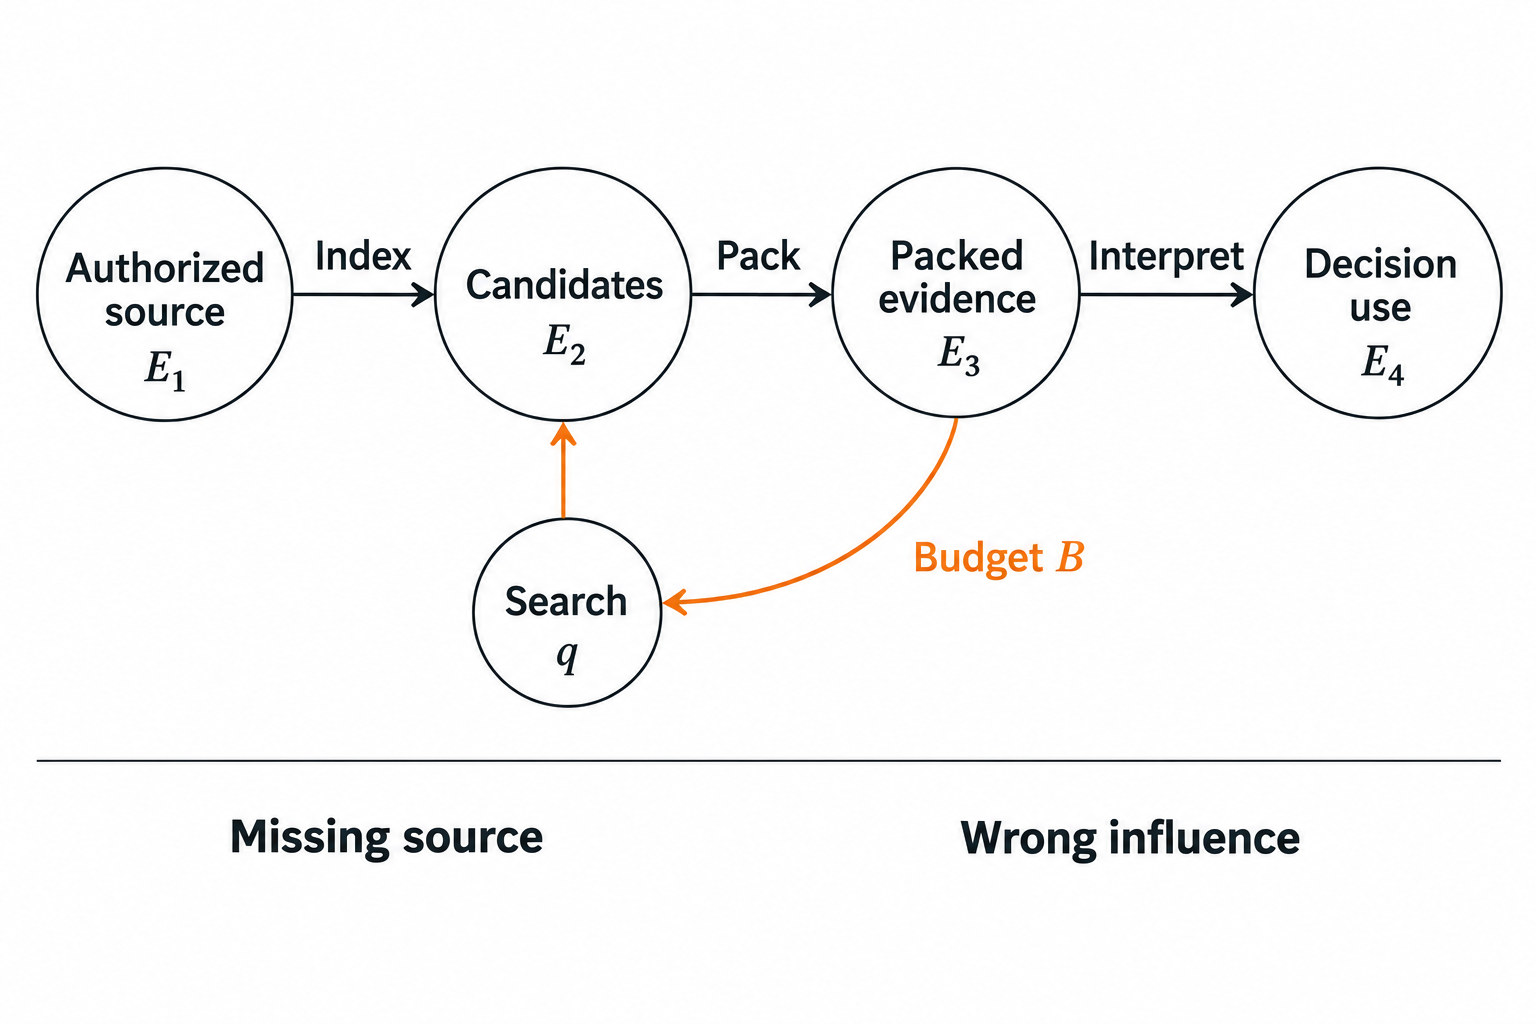
\includegraphics[width=\linewidth]{book/figures/assets/F16review.png}
\caption{A decisive-evidence path with separate failure boundaries. Authorized source availability, candidate selection, qualified packing and appropriate use are nested events for this specified path. Conditional stage probabilities multiply without an independence assumption. Alternative valid evidence paths may still solve the task. A return to search is a policy choice with cost; it does not establish evidence sufficiency.}
\label{fig:C16:overview}
\end{figure}
